\documentclass{standalone}
\usepackage{tikz}
\begin{document}
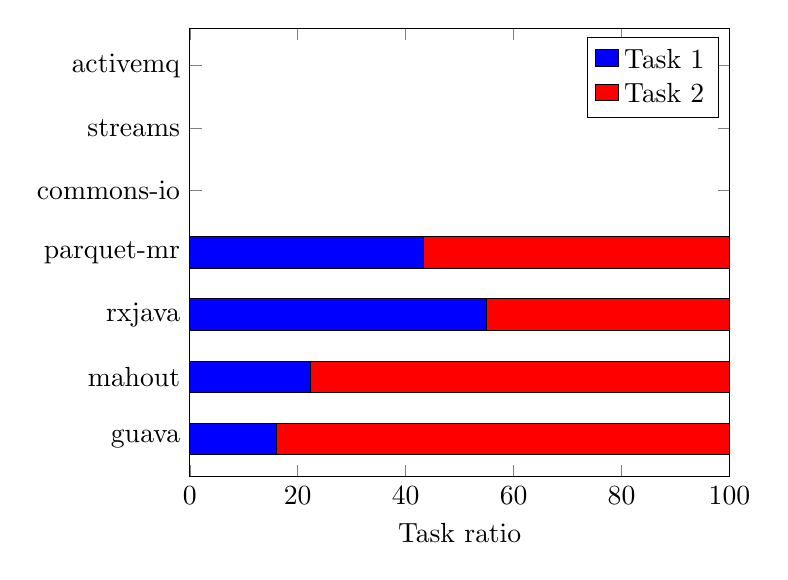
\begin{tikzpicture}
  \begin{axis}[
    xbar stacked, xmin=0, xmax=100,
    xlabel={Task ratio},
    bar width=4mm,
    symbolic y coords={guava,mahout,rxjava,parquet-mr, commons-io, streams, activemq},
    ytick=data
  ]
\addplot [fill=blue] coordinates {
    (16.07,guava)
    (22.4,mahout)
    (55.06,rxjava)
    (43.38,parquet-mr)
    (0,commons-io)
    (0,streams)
    (0,activemq)};
\addplot [fill=red] coordinates {
    (83.93,guava)
    (77.6,mahout)
    (44.94,rxjava)
    (56.62,parquet-mr)
    (0,commons-io)
    (0,streams)
    (0,activemq)};
\legend{Task 1,Task 2}
\end{axis}
\end{tikzpicture}
\end{document}
